Table~\ref{fig:reducedr2} shows reduced rank $2$ root systems.
These are the only reduced rank $2$ root systems.
Of these, $A_1$, $B_2$ and $G_2$ are irreducible and $A_1\times A_1$ is reducible.

\begin{table}[h]
	\centering
	\begin{tabular}{@{}cl@{}} \toprule
	Picture & Description \\ \midrule
		\adjustbox{valign=t}{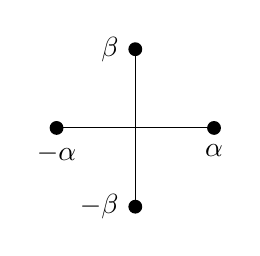
\begin{tikzpicture}[dot/.style={circle, fill, inner sep=0pt, outer sep=0pt, minimum size=5pt}]
		\draw (-1, 0) -- (1, 0);
		\draw (0, -1) -- (0, 1);
			\node[dot, label=below:$-\alpha$] at (-1, 0) {};
			\node[dot, label=below:$\alpha$] at (1, 0) {};
			\node[dot, label=left:$\beta$] at (0, 1) {};
			\node[dot, label=left:$-\beta$] at (0, -1) {};
		\end{tikzpicture}} &%
	\adjustbox{valign=t}{\begin{minipage}{0.5\textwidth}%
		\begin{itemize}[left=0pt, topsep=0pt, noitemsep]
			\item type $A_1\times A_1$
			\item arising from $\mathfrak{sl}_2\times \mathfrak{sl}_2$
			\item not irreducible
			\item Weyl group $C_2\times C_2$
		\end{itemize}
	\end{minipage}} \\ \midrule
		\adjustbox{valign=t}{\begin{tikzpicture}[dot/.style={circle, fill, inner sep=0pt, outer sep=0pt, minimum size=5pt}]
			\node[dot, label=below:$\alpha$] (a) at (1, 0) {};
			\node[dot, label=left:$\beta$] (b) at (120:1) {};
			\node[dot, label=right:$\beta+\alpha$] (ab) at ($ (a) + (b) $) {};
			\node[dot, label=below:$-\alpha$] (ma) at ($ (0, 0) - (a) $) {};
			\node[dot, label=right:$-\beta$] (mb) at ($ (0, 0) - (b) $) {};
			\node[dot, label=left:$-\beta-\alpha$] (mab) at ($ (0, 0) - (ab) $) {};
			\draw (ma) -- (a);
			\draw (mb) -- (b);
			\draw (mab) -- (ab);
		\end{tikzpicture}} &%
	\adjustbox{valign=t}{\begin{minipage}{0.5\textwidth}%
		\begin{itemize}[left=0pt, topsep=0pt, noitemsep]
			\item type $A_2$
			\item arising from $\mathfrak{sl}_3$ (TODO: why? CSA are diagonal
				matrices)
			\item $\alpha^\vee = \alpha$, $\beta^\vee = \beta$
			\item $(\alpha, \beta) = -1$
			\item $\dim \mathfrak{sl}_3 = 6 + 2$, where $6$ is the number of roots
				and $2$ is the rank (this comes from the Cartan decomposition!)
			\item Weyl group $D_6 \cong S_3$
		\end{itemize}
	\end{minipage}}\\ \midrule
		\adjustbox{valign=t}{\begin{tikzpicture}[dot/.style={circle, fill, inner sep=0pt, outer sep=0pt, minimum size=5pt}]
			\node[dot, label=below:$\alpha$] (a) at (1, 0) {};
			\node[dot, label=left:$\beta$] (b) at (-1, 1) {};
			\node[dot, label=above:$\beta+\alpha$] (ab) at ($ (a) + (b) $) {};
			\node[dot, label=right:$\beta+2\alpha$] (aab) at ($ (a) + (ab) $) {};
			\node[dot, label=below:$-\alpha$] (ma) at ($ (0, 0) - (a) $) {};
			\node[dot, label=right:$-\beta$] (mb) at ($ (0, 0) - (b) $) {};
			\node[dot, label=below:$-\beta-\alpha$] (mab) at ($ (0, 0) - (ab) $) {};
			\node[dot, label=left:$-\beta-2\alpha$] (maab) at ($ (0, 0) - (aab) $) {};
			\draw (ma) -- (a);
			\draw (mb) -- (b);
			\draw (mab) -- (ab);
			\draw (maab) -- (aab);
		\end{tikzpicture}} &%
	\adjustbox{valign=t}{\begin{minipage}{0.5\textwidth}%
		\begin{itemize}[left=0pt, topsep=0pt, noitemsep]
			\item type $B_2$
			\item $(\alpha, \alpha) = 1$, $(\beta, \beta) = 2$
			\item arises from $\mathfrak{sp}_4$ and $\mathfrak{so}_5$
			\item $\dim L = 10 = 8 + 2$
		\end{itemize}
	\end{minipage}} \\ \midrule
		\adjustbox{valign=t}{\begin{tikzpicture}[dot/.style={circle, fill, inner sep=0pt, outer sep=0pt, minimum size=5pt}]
			\node[dot, label=right:$\alpha$] (a) at (1, 0) {};
			\node[dot, label=left:$\beta$] (b) at (150:1.7320508) {};
			\node[dot, label=above left:$\beta+\alpha$] (ab) at ($ (a) + (b) $) {};
			\node[dot, label=above right:$\beta+2\alpha$] (aab) at ($ (a) + (ab) $) {};
			\node[dot, label=right:$\beta+3\alpha$] (aaab) at ($ (a) + (aab) $) {};
			\node[dot, label=left:$-\alpha$] (ma) at ($ (0, 0) - (a) $) {};
			\node[dot, label=right:$-\beta$] (mb) at ($ (0, 0) - (b) $) {};
			\node[dot, label=below right:$-\beta-\alpha$] (mab) at ($ (0, 0) - (ab) $) {};
			\node[dot, label=below left:$-\beta-2\alpha$] (maab) at ($ (0, 0) - (aab) $) {};
			\node[dot, label=left:$-\beta-3\alpha$] (maaab) at ($ (0, 0) - (aaab) $) {};
			\node[dot, label=above: $2\beta + 3\alpha$]  (to) at (90:1.7320508) {};
			\node[dot, label=below: $-2\beta -3\alpha$] (bo) at (270:1.7320508) {};
			\draw (maaab) -- (to) -- (mb) -- (maaab);
			\draw (aaab) -- (bo) -- (b) -- (aaab);
		\end{tikzpicture}} &%
	\adjustbox{valign=t}{\begin{minipage}{0.5\textwidth}%
		\begin{itemize}[left=0pt, topsep=0pt, noitemsep]
			\item type $G_2$
			\item arising from the Lie algebra of derivations of the octionions
			\item Weyl group is dihedral $D_{12}$ of order $12$
		\end{itemize}
	\end{minipage}} \\ \bottomrule
\end{tabular}
\caption{Reduced rank $2$ root systems}
\label{fig:reducedr2}
\end{table}
